\documentclass[11pt,class=report,crop=false]{standalone}
\usepackage[screen]{../python}



\begin{document}


%====================================================================
\chapitre{Transformée de Fourier discrète}
%====================================================================


\insertvideo{6h0c2jMuHUg}{partie 15. Transformée de Fourier discrète (par des dessins)}


\objectifs{Nous revenons sur l'outil principal de l'algorithme de Shor : la transformée de Fourier. Nous expliquons comment elle est construite, comment la réaliser par un circuit quantique et quelles sont ses autres applications.}

\index{transformee de Fourier@transformée de Fourier}

%%%%%%%%%%%%%%%%%%%%%%%%%%%%%%%%%%%%%%%%%%%%%%%%%%%%%%%%%%%%%%%%%%%%%
\section{Comprendre la transformée de Fourier}

La transformée de Fourier, c'est la magie de pouvoir récupérer chacune des couleurs qu'on a mélangées dans un pot de peinture !

%--------------------------------------------------------------------
\subsection{Les transformées de Fourier}

\begin{center}
    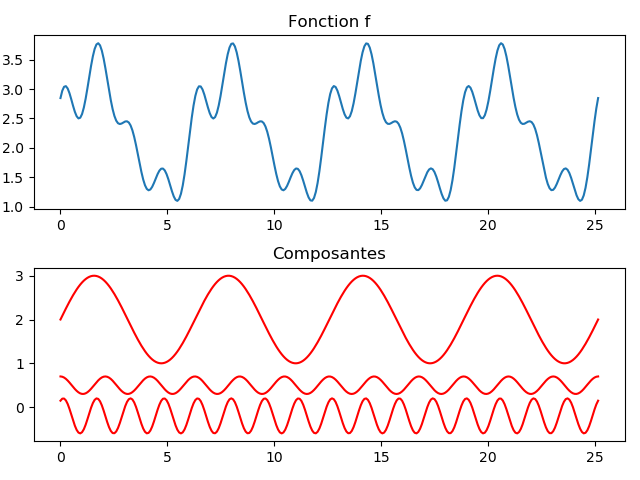
\includegraphics[scale=\myscale,scale=0.7]{figures/fourier-1}
\end{center}

Voici un exemple : on prend trois fonctions sinusoïdales $f_1, f_2, f_3$ (figure du bas) que l'on additionne pour obtenir une fonction compliquée $f(x) = f_1(x) + f_2(x) + f_3(x)$ (figure du haut). Alors la transformée de Fourier permet de retrouver chacune des composantes $f_1, f_2, f_3$ à partir de $f$.

\bigskip

Le monde de Fourier est assez vaste, voici un petit lexique :
\begin{itemize}
  \item la transformée de Fourier concerne une fonction quelconque, elle se calcule à l'aide d'une intégrale,
  \item les séries de Fourier s'appliquent à des fonctions périodiques (comme ci-dessus),
  \item la transformée de Fourier discrète s'applique à une liste de nombres réels ou complexes,
  \item la transformée de Fourier discrète quantique est une variante de la précédente et transforme un qubit en un autre qubit.
\end{itemize}



%--------------------------------------------------------------------
\subsection{La transformée de Fourier discrète classique}

Nous allons expliquer le principe de la transformée de Fourier discrète (non quantique) et justifier comment elle permet de retrouver les périodes.

Voici la définition de la transformée de Fourier discrète.
Soit $(x_0,\ldots,x_{n-1})$  une suite de $n$ nombres (ils peuvent être complexes mais pour nos exemples ce seront des réels).
La transformée de Fourier discrète de $(x_0,\ldots,x_{n-1})$ est la liste de nombres complexes $(X_0,\ldots, X_{n-1})$ où chaque $X_k$ est défini par :
\mybox{$\displaystyle
X_k = \frac{1}{\sqrt n}\sum_{j=0}^{n-1} x_j e^{-2\ii\pi \frac{k \cdot j}{n}}.$}
Si on note $\omega = e^{\frac{2\ii\pi}{n}}$ et $\omega^*= e^{-\frac{2\ii\pi}{n}}$,
alors
$$X_k = \frac{1}{\sqrt n} \left( x_0(\omega^*)^{k\cdot 0} + x_1(\omega^*)^{k\cdot 1} +
\cdots +  x_{n-1}(\omega^*)^{k \cdot (n-1)}\right).$$

La formule n'est donc pas si difficile à comprendre.  Mais pourquoi vouloir transformer une suite de nombres par une opération aussi compliquée ?

%--------------------------------------------------------------------
\subsection{Construction de la transformée de Fourier discrète}

L'idée de la construction de la transformée de Fourier est très simple !
Nous avons des données $x_j$ (pour nous $x_j \in \Rr$). Nous représentons traditionnellement $x_j$ sous la forme d'un point (où l'ordonnée du point est la valeur $x_j$, les points étant placés de gauche à droite). Mais on peut aussi utiliser une représentation circulaire : chaque point est à une distance $x_j$ de l'origine, et les points sont répartis dans le sens des aiguilles d'une montre. 


\begin{center}
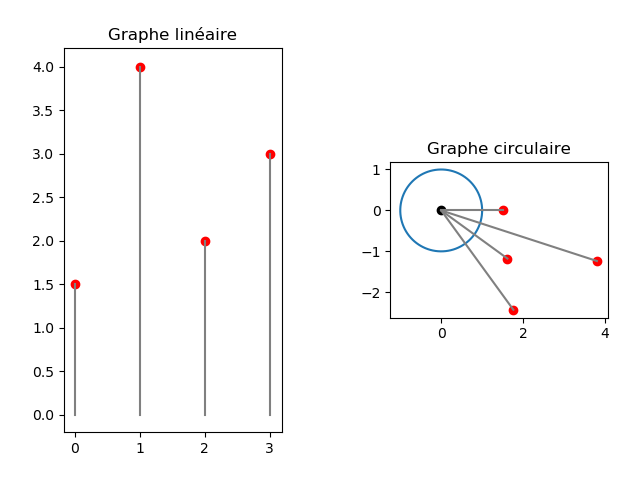
\includegraphics[scale=\myscale,scale=0.7]{figures/fourier-2}

\nopagebreak

\begin{minipage}{0.8\textwidth}
\center\emph{
Les données sont $(x_0,x_1,x_2,x_3) = (1.5,4,2,3).$\\
Figure de gauche : les données sont présentées sous la forme de points $(j,x_j)$.\\
Figure de droite les mêmes données sous forme d'écriture polaire : l'angle est proportionnel à $j$ et le rayon est $x_j$.}
\end{minipage}

\end{center}

Le point clé de la représentation circulaire est qu'on peut répartir les données sur un angle plus ou moins grand. Notons $2\pi t$ l'angle total d'étalement, alors plus précisément l'angle entre deux données est $\frac{2\pi t}{n}$.

Comment est calculée cette représentation circulaire ? La donnée $x_j$ correspond au point du plan situé à distance $x_j$ de l'origine et faisant un angle $-\frac{2\pi t}{n} \times j$ avec l'horizontale : c'est donc le nombre complexe $z_j = x_j e^{-2 \ii \pi \frac{t}{n} j}$. On voit apparaître le terme de la définition de la transformée de Fourier.


Voici différents étalements possibles, ils correspondent à différentes valeurs du paramètre $t$.
Pour $t=\frac14$ les données sont réparties sur un quart de cercle, pour $t=\frac12$ un demi-cercle, pour $t=1$ le cercle entier et pour $t>1$ les données s'enroulent plusieurs fois autour du cercle.


\begin{center}
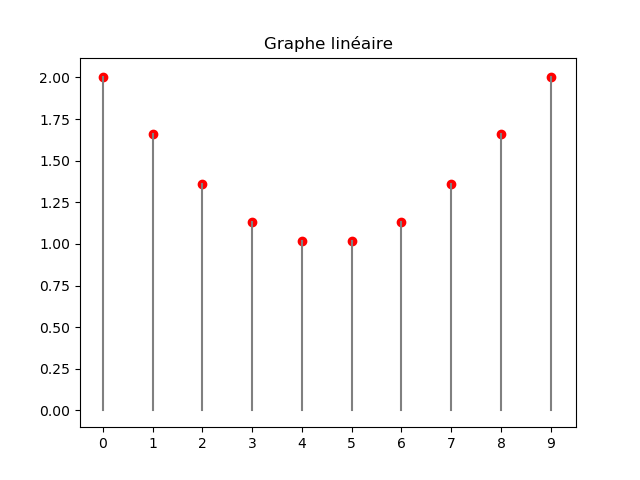
\includegraphics[scale=\myscale,scale=0.5]{figures/fourier-3a}

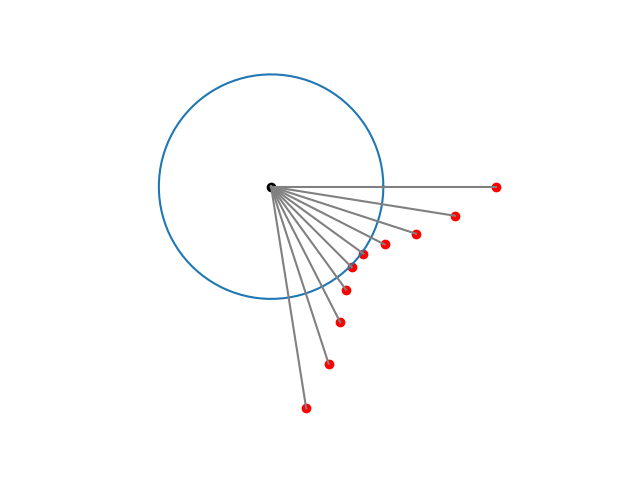
\includegraphics[scale=\myscale,scale=0.4]{figures/fourier-3b}
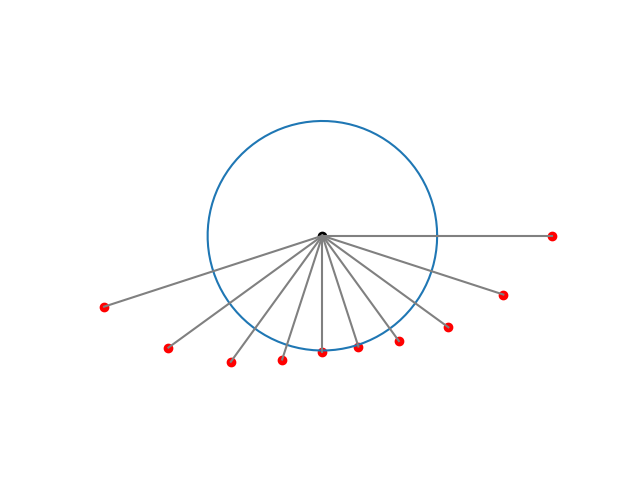
\includegraphics[scale=\myscale,scale=0.4]{figures/fourier-3c}

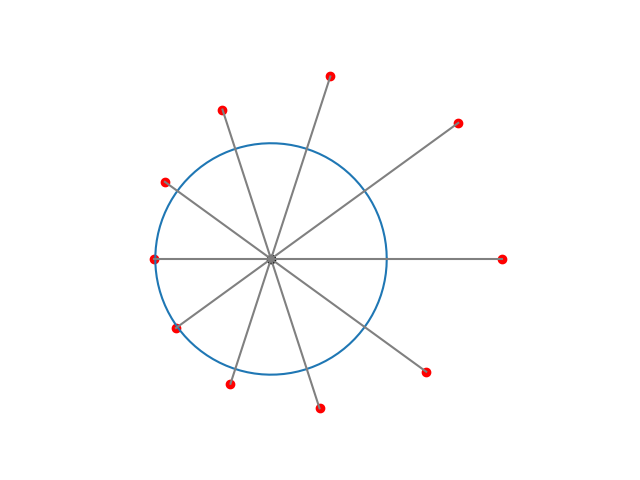
\includegraphics[scale=\myscale,scale=0.4]{figures/fourier-3d}
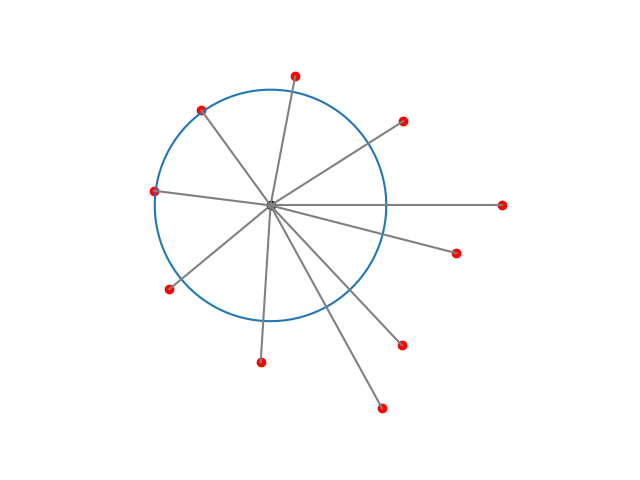
\includegraphics[scale=\myscale,scale=0.4]{figures/fourier-3e}

\nopagebreak

\begin{minipage}{0.8\textwidth}
\center\emph{
Figure de dessus : les données sont sous la forme de points $(j,x_j)$.\\
Figures du dessous : les mêmes données sous forme circulaire avec $t=\frac14$, $t=\frac12$, $t=1$~et~$t>1$.}
\end{minipage}

\end{center}


%--------------------------------------------------------------------
\subsection{Enroulements particuliers}

On remplace l'étude d'une fonction $f : [a,b] \to \Rr$ par l'étude de valeurs $x_j=f(a_j)$ pour une subdivision $(a_j)$ de l'intervalle $[a,b]$. Pour avoir une meilleure précision, il suffit d'augmenter le nombre $n$ de points dans la subdivision.
On relie les points de ces données pour approcher le graphe de $f$.

\begin{center}
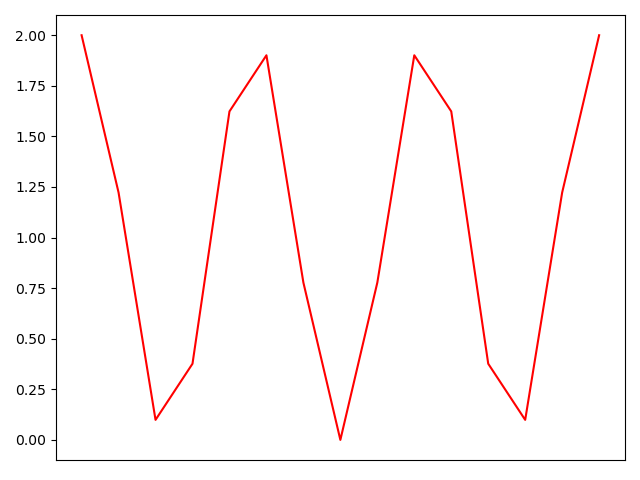
\includegraphics[scale=\myscale,scale=0.33]{figures/fourier-4a}
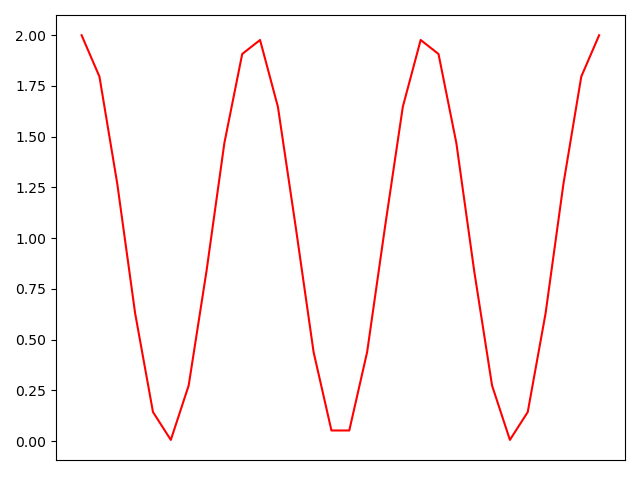
\includegraphics[scale=\myscale,scale=0.33]{figures/fourier-4b}
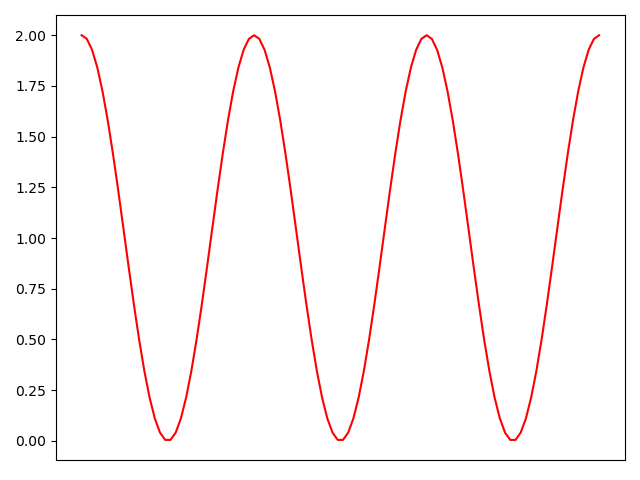
\includegraphics[scale=\myscale,scale=0.33]{figures/fourier-4c}


\nopagebreak

\begin{minipage}{0.8\textwidth}
\center\emph{
Fonction $f(x) = 1+\cos(3x)$ sur l'intervalle $[0,2\pi]$.\\
Les données sont les $x_j = f(a_j)$ avec une subdivision de $n=15$ points à gauche,\\
$n=30$ au centre, $n=100$ à droite. %Les points sont reliés entre eux.
}
\end{minipage}

\end{center}

On peut aussi relier les points du graphe circulaire. Géométriquement on a ainsi enroulé le graphe de la fonction $f$, sur le cercle.

\begin{center}
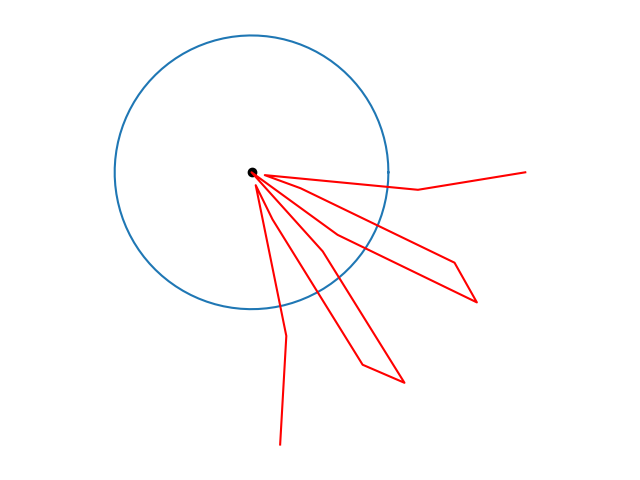
\includegraphics[scale=\myscale,scale=0.33]{figures/fourier-5a}
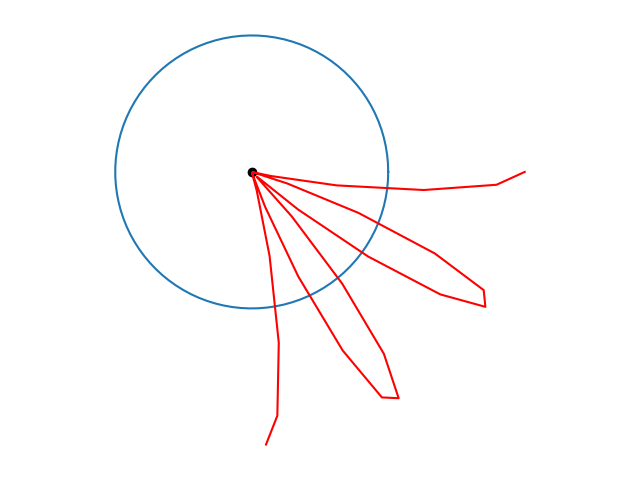
\includegraphics[scale=\myscale,scale=0.33]{figures/fourier-5b}
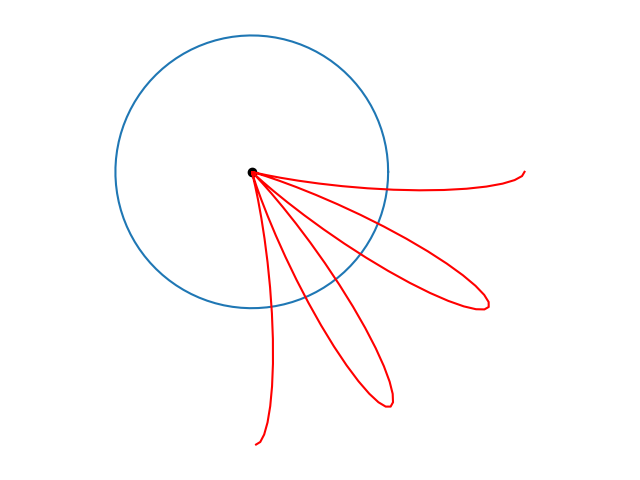
\includegraphics[scale=\myscale,scale=0.33]{figures/fourier-5c}

\begin{minipage}{0.8\textwidth}
\center\emph{
Les mêmes données sur le graphe circulaire avec $n=15$ points à gauche,\\
$n=30$ au centre, $n=100$ à droite. %Les points sont reliés entre eux.
}
\end{minipage}

\end{center}



Regardons maintenant les différents enroulements selon le paramètre d'étalement $t$. 
Tout d'abord on exclut les $t$ avec $t<1$ car le graphe ne s'enroule pas totalement autour du cercle. 
Pour la plupart des paramètres on obtient une jolie figure symétrique autour de l'origine, mais il y a des exceptions. 
Pour $t=3$ on obtient une figure complètement décalée à droite. Que se passe-t-il en $t=3$ ? Le graphe de $f$ est périodique et pour cette valeur de $t$ la courbe enroulée vient se superposer à elle-même lors des enroulements successifs.


\begin{center}
	\begin{minipage}{0.24\textwidth}
	\center 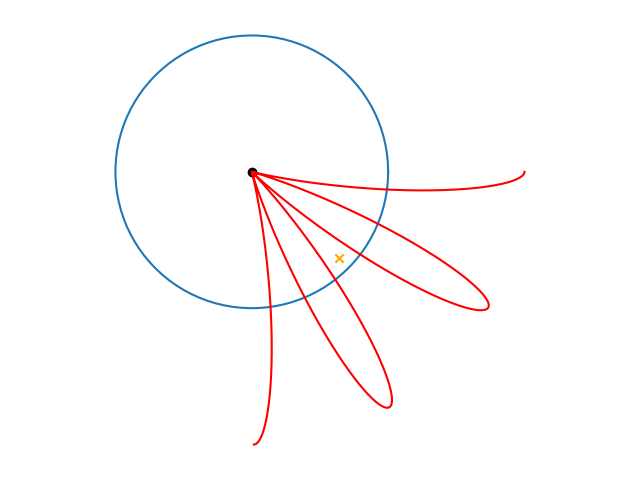
\includegraphics[scale=\myscale,scale=0.3]{figures/fourier-6-025}
	$t = 0.25$ 
	\end{minipage}
	\begin{minipage}{0.24\textwidth}
	\center 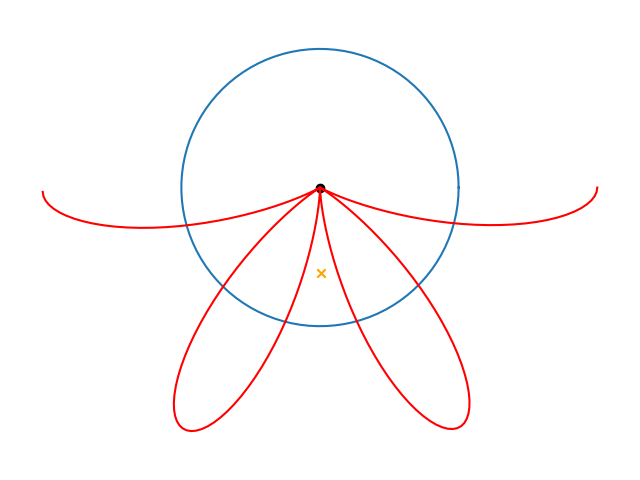
\includegraphics[scale=\myscale,scale=0.3]{figures/fourier-6-050}
	$t = 0.5$ 
	\end{minipage}
	\begin{minipage}{0.24\textwidth}
	\center 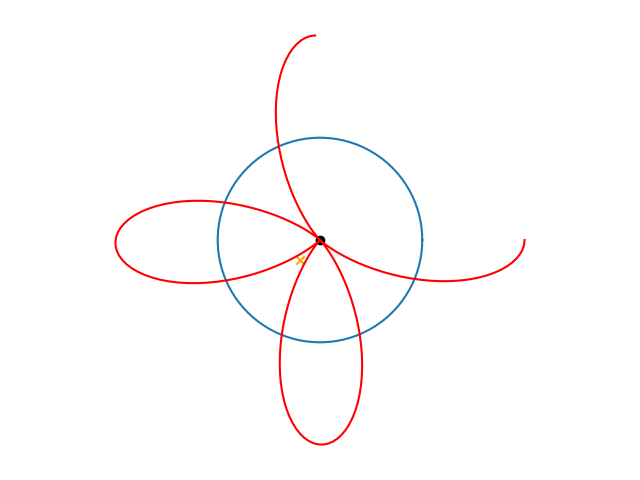
\includegraphics[scale=\myscale,scale=0.3]{figures/fourier-6-075}
	$t = 0.75$ 
	\end{minipage}
	\begin{minipage}{0.24\textwidth}
	\center 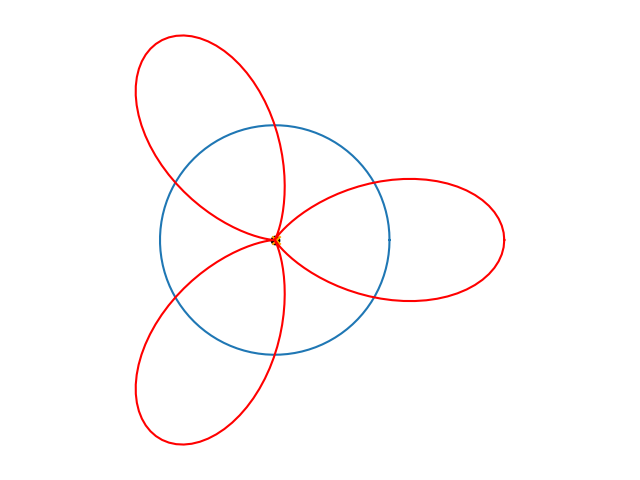
\includegraphics[scale=\myscale,scale=0.3]{figures/fourier-6-100}
	$t = 1$ 
	\end{minipage}


	\begin{minipage}{0.23\textwidth}
	\center 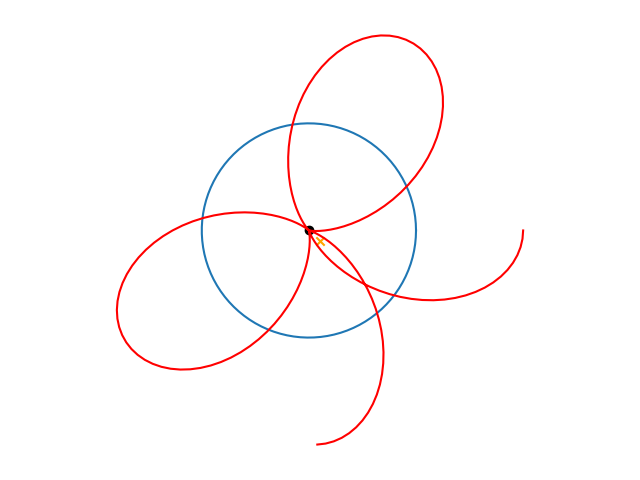
\includegraphics[scale=\myscale,scale=0.3]{figures/fourier-6-125}
	$t = 1.25$ 
	\end{minipage}
	\begin{minipage}{0.27\textwidth}
	\center 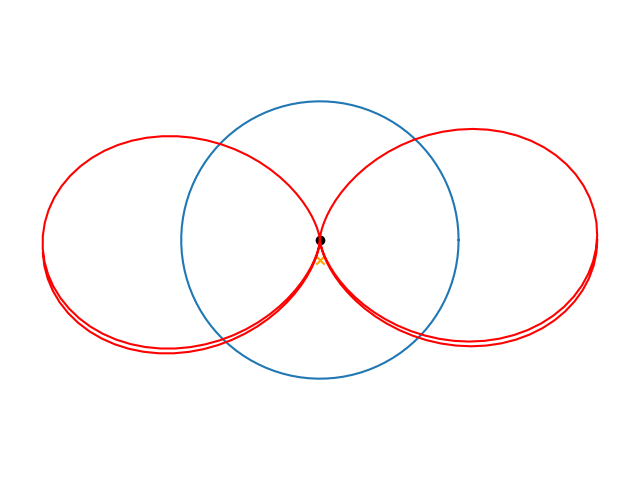
\includegraphics[scale=\myscale,scale=0.3]{figures/fourier-6-150}
	$t = 1.50$ 
	\end{minipage}
	\begin{minipage}{0.24\textwidth}
	\center 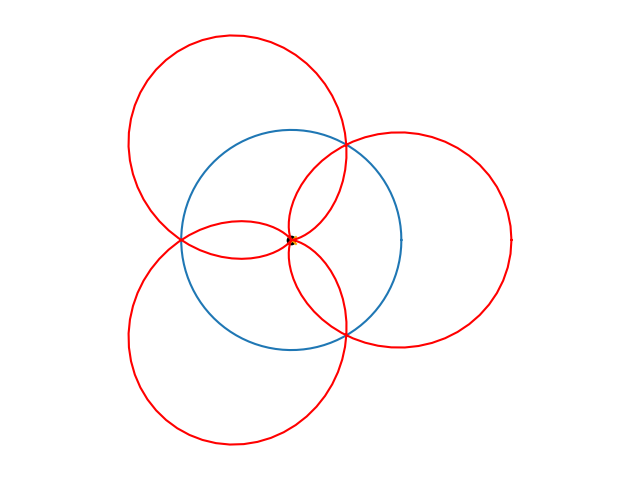
\includegraphics[scale=\myscale,scale=0.3]{figures/fourier-6-200}
	$t = 2$ 
	\end{minipage}
	\begin{minipage}{0.24\textwidth}
	\center 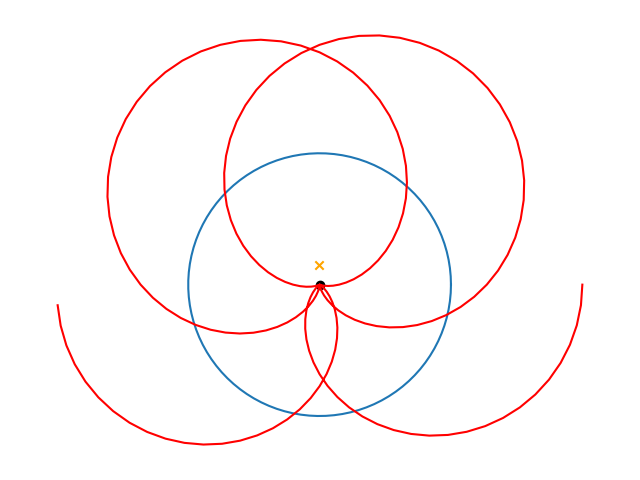
\includegraphics[scale=\myscale,scale=0.3]{figures/fourier-6-250}
	$t = 2.5$ 
	\end{minipage}

	\begin{minipage}{0.25\textwidth}
	\center 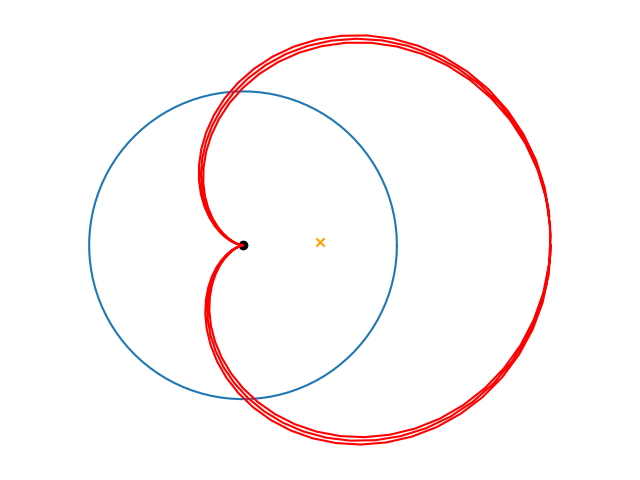
\includegraphics[scale=\myscale,scale=0.3]{figures/fourier-6-300}
	$t = 3$ 
	\end{minipage}
	\begin{minipage}{0.25\textwidth}
	\center 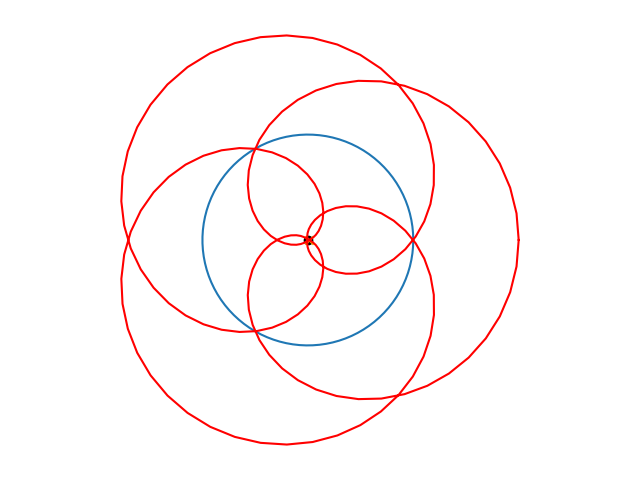
\includegraphics[scale=\myscale,scale=0.3]{figures/fourier-6-400}
	$t = 4$ 
	\end{minipage}
	\begin{minipage}{0.25\textwidth}
	\center 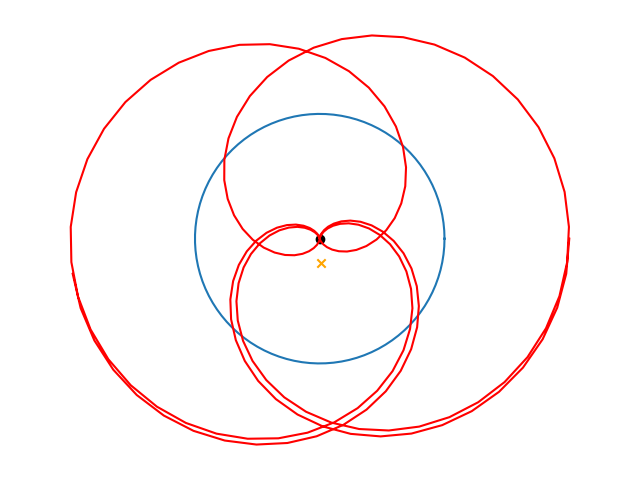
\includegraphics[scale=\myscale,scale=0.3]{figures/fourier-6-450}
	$t = 4.5$ 
	\end{minipage}
	\begin{minipage}{0.23\textwidth}
	\center 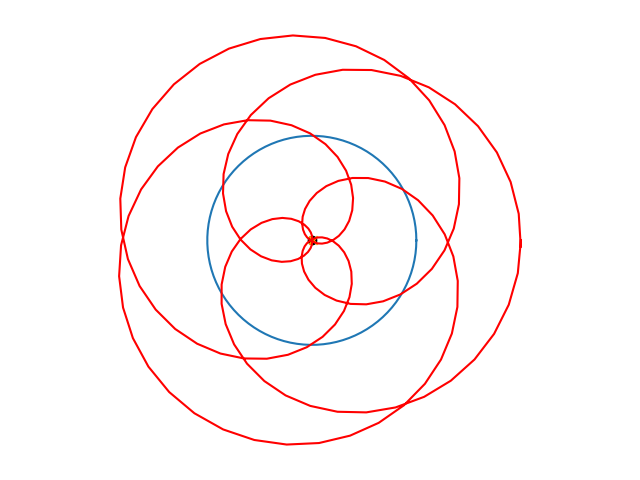
\includegraphics[scale=\myscale,scale=0.3]{figures/fourier-6-500}
	$t = 5$ 
	\end{minipage}

\medskip

\nopagebreak


\begin{minipage}{0.8\textwidth}
  \center\emph{Graphe de $f(x) = 1+\cos(3x)$ sur l'intervalle $[0,2\pi]$\\
    enroulé sur le cercle pour différentes valeurs de $t$.\\
    Pour $t=3$ la figure n'est plus symétrique par rapport à l'origine.\\
    La petite croix\couleurnb{ orange}{} désigne le centre de gravité.
}
\end{minipage}

\end{center}

Ce cas particulier $t=3$ est le cas qui nous intéresse ! Le paramètre $t=3$ correspond à la période de notre fonction. En effet, la fonction $f(x) = 1 + \cos(3x)$ est $\frac{2\pi}{3}$ périodique et le paramètre spécial est $t=3$.
Pour une fonction $f(x) = 1 + \cos(\alpha x)$, la période est $\frac{2\pi}{\alpha}$ et le paramètre spécial est $t=\alpha$ (en fait $t$ correspond à la fréquence qui est l'inverse de la période). 






%--------------------------------------------------------------------
\subsection{Centre de gravité}


Est-ce que cette technique permet d'obtenir les différentes périodes d'un signal obtenu par superposition (comme dans l'exemple du tout début de ce chapitre) ? La réponse est oui !
Voyons comment repérer ces paramètres particuliers qui correspondent à des périodes.
Pour la plupart des paramètres les figures obtenues sont symétriques par rapport à l'origine, donc le centre de gravité est proche de l'origine (en physique on parle d'interférence destructive). Par contre, pour certains paramètres particuliers, le centre de gravité s'éloigne de l'origine. Nous obtenons donc un critère numérique simple.

Le centre de gravité des points se calcule comme une moyenne des points :
$$X_t = \frac{1}{\sqrt n}\sum_{j=0}^{n-1} x_j e^{-2\ii\pi \frac{t \cdot j}{n}}.$$

Quelques remarques :
\begin{itemize}
  \item Sur les dessins précédents ce centre de gravité était représenté par une petite croix\couleurnb{ orange}{}.
  \item Nous préférons le choix du coefficient $\frac{1}{\sqrt n}$  (au lieu du coefficient $\frac1n$ du vrai centre de gravité).
  \item Pour $t=k$ la formule est exactement celle de la transformée de Fourier discrète des $(x_j)$.
\end{itemize}

Comment évolue $X_t$ en fonction de $t$ et comment repérer les paramètres particuliers ?
Le nombre $X_t$ est un nombre complexe, on se contente de regarder sa partie réelle
$\Re(X_t)$. La fonction $t \mapsto \Re(X_t)$ mesure donc l'abscisse du centre de gravité.


\begin{center}
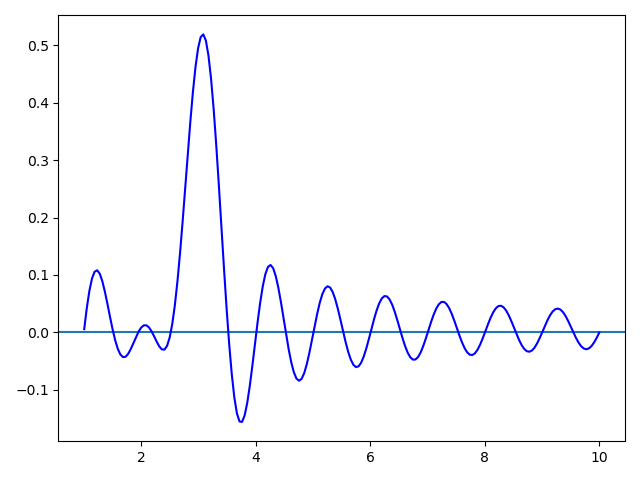
\includegraphics[scale=\myscale,scale=0.5]{figures/fourier-7}

\nopagebreak

\begin{minipage}{0.8\textwidth}
\center\emph{Graphe de la fonction $t \mapsto \Re(X_t)$ qui mesure l'abscisse du centre de gravité de l'enroulement de la fonction $f(x) = 1+\cos(3x)$ sur l'intervalle $[0,2\pi]$ pour différentes valeurs de $t$. Le pic à $t=3$ marque la rupture de symétrie.
}
\end{minipage}
\end{center}


Pour la plupart des valeurs de $t$, $\Re(X_t)$ est proche de $0$, les pics correspondent à la rupture de symétrie centrale et déterminent les périodes des composantes de la fonction.

%--------------------------------------------------------------------
\subsection{Autre exemple}

Soient $f_1(x) = 1 + \cos(3x)$ et $f_2(x) = \frac12(1+\cos(5x))$ et leur somme $f(x) = f_1(x) + f_2(x)$ définie sur l'intervalle $[0,2\pi]$. \`A partir de $f$, nous souhaitons retrouver les périodes $\frac{2\pi}{3}$ et $\frac{2\pi}{5}$ de ses deux composantes.


\begin{center}
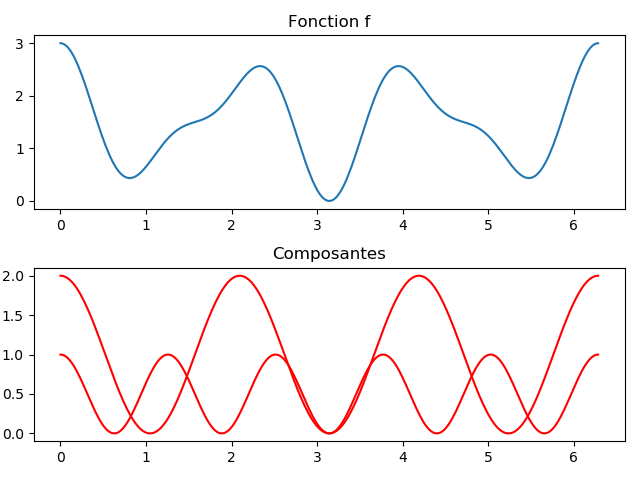
\includegraphics[scale=\myscale,scale=0.5]{figures/fourier-8bis}

\nopagebreak

\begin{minipage}{0.8\textwidth}
\center\emph{Le graphe de la fonction $f(x) =  f_1(x) + f_2(x)$ sur $[0,2\pi]$\\ avec $f_1(x) = 1 + \cos(3x)$ et $f_2(x) = \frac12(1+\cos(5x))$.
}
\end{minipage}
\end{center}

On enroule le graphe de $f$ sur un cercle, selon différentes valeurs de $t$.

\begin{center}
	\begin{minipage}{0.26\textwidth}
	\center 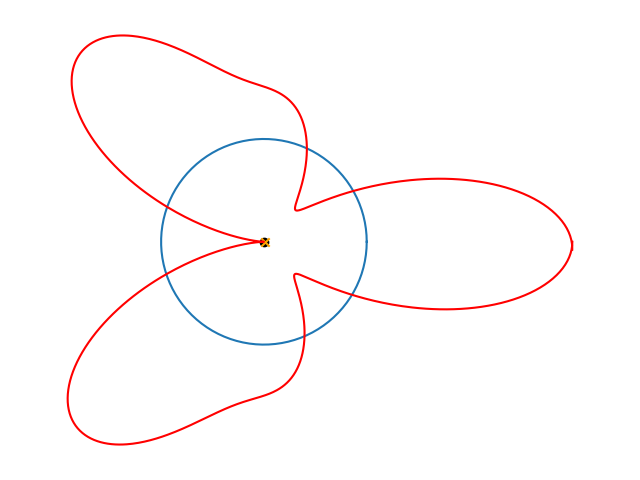
\includegraphics[scale=\myscale,scale=0.3]{figures/fourier-9-1}
	$t = 1$ 
	\end{minipage}
	\begin{minipage}{0.24\textwidth}
	\center 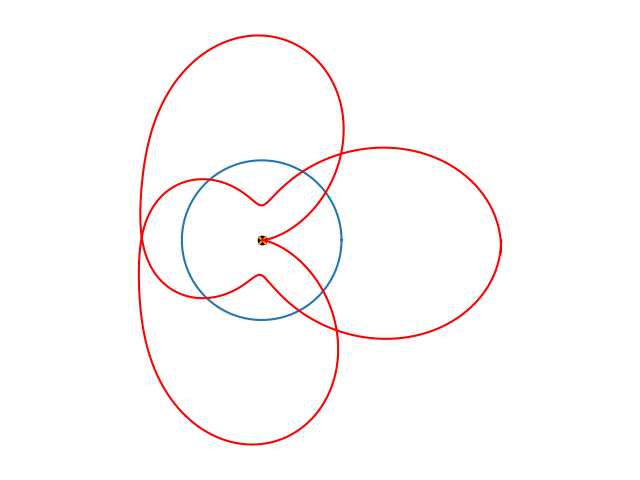
\includegraphics[scale=\myscale,scale=0.3]{figures/fourier-9-2}
	$t = 2$ 
	\end{minipage}
	\begin{minipage}{0.24\textwidth}
	\center 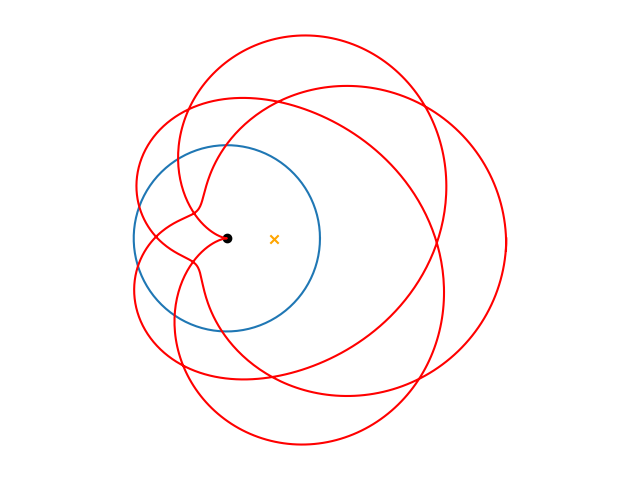
\includegraphics[scale=\myscale,scale=0.3]{figures/fourier-9-3}
	$t = 3$ 
	\end{minipage}
	\begin{minipage}{0.24\textwidth}
	\center 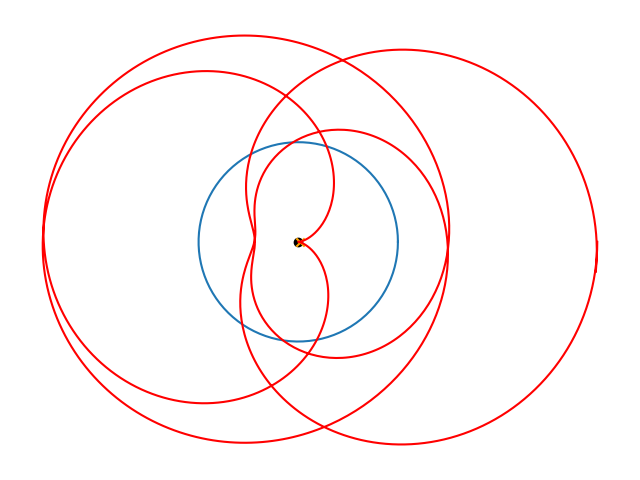
\includegraphics[scale=\myscale,scale=0.3]{figures/fourier-9-4}
	$t = 4$ 
	\end{minipage}


	\begin{minipage}{0.3\textwidth}
	\center 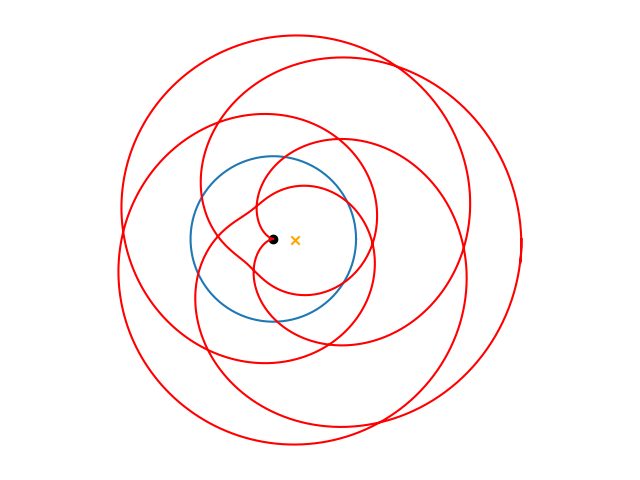
\includegraphics[scale=\myscale,scale=0.33]{figures/fourier-9-5}
	$t = 5$ 
	\end{minipage}
	\begin{minipage}{0.3\textwidth}
	\center 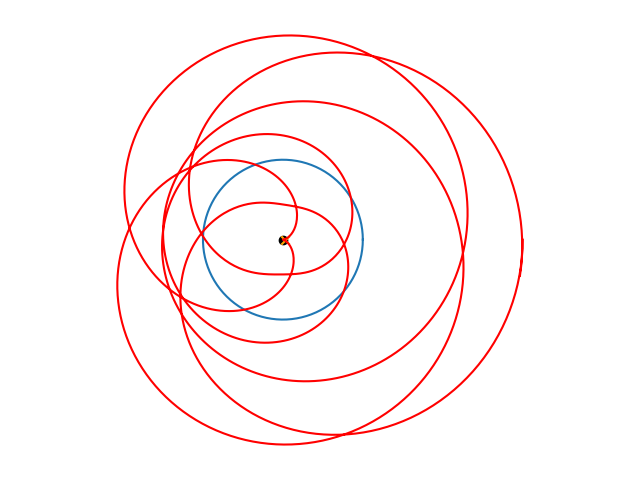
\includegraphics[scale=\myscale,scale=0.33]{figures/fourier-9-6}
	$t = 6$ 
	\end{minipage}
	\begin{minipage}{0.3\textwidth}
	\center 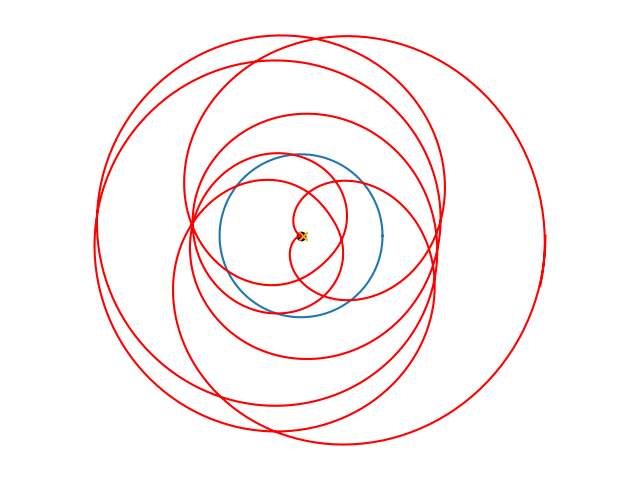
\includegraphics[scale=\myscale,scale=0.33]{figures/fourier-9-7}
	$t = 7$ 
	\end{minipage}

\medskip

\nopagebreak

\begin{minipage}{0.8\textwidth}
\center\emph{Enroulement du graphe de $f$ pour différentes valeurs de $t$.\\  Noter le décalage du  centre de gravité (la croix\couleurnb{ orange}{}) en $t=3$ et $t=5$.
}
\end{minipage}

\end{center}

Le centre de gravité se calcule selon la formule de la transformée de Fourier discrète, pour nos paramètres $t=1,t=2,\ldots$ 
$$X_t = \frac{1}{\sqrt n}\sum_{j=0}^{n-1} x_j e^{-2\ii\pi \frac{t \cdot j}{n}}.$$
où $x_j = f\left(\frac{j}{n}\right)$

\begin{center}
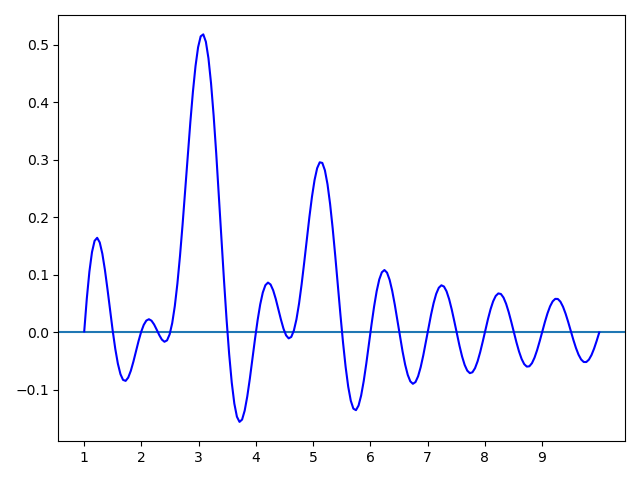
\includegraphics[scale=\myscale,scale=0.5]{figures/fourier-10}

\nopagebreak

\begin{minipage}{0.8\textwidth}
\center\emph{Graphe de la fonction $t \mapsto \Re(X_t)$ qui mesure l'abscisse du centre de gravité de l'enroulement de la fonction $f(x)$ sur l'intervalle $[0,2\pi]$ pour différentes valeurs de $t$.\\ On remarque des pics en $t=3$ et $t=5$.
}
\end{minipage}
\end{center}


%--------------------------------------------------------------------
\subsection{L'inverse de la transformée de Fourier discrète}

On a donc vu l'intérêt de la transformée de Fourier : elle permet de retrouver les caractéristiques d'une fonction (ou d'une série de données). Mais de plus cette transformation ne perd pas d'information. D'un point de vue mathématique la transformation est bijective. On peut retrouver les $(x_k)$ connaissant les $(X_j)$ par une formule similaire (seul le signe de l'exponentielle change) :

$$x_k = \frac{1}{\sqrt n}\sum_{j=0}^{n-1} X_j e^{+2\ii\pi \frac{k \cdot j}{n}}.$$


Conclusion : la transformée de Fourier discrète transforme une liste de $n$ nombres en  une autre liste de $n$ nombres. Cette transformation est bijective et permet en particulier de déterminer la période d'un signal périodique.

%--------------------------------------------------------------------
\subsection{La transformée de Fourier discrète quantique}

La transformée de Fourier discrète quantique est par définition cette variante de la transformée de Fourier discrète :
$$\hat F \ket{\underline k} = \frac{1}{\sqrt{2^n}} \sum_{j=0}^{2^n-1} e^{2\ii \pi \frac{k \cdot j}{2^n}} \ket{\underline j}$$

Les différences sont les suivantes :
\begin{itemize}
  \item Par convention on choisit un signe \og{}$+$\fg{} pour l'exposant de la transformée quantique (comme pour la transformée de Fourier discrète \emph{inverse} classique).

  \item Les données sont remplacées par les qubits de bases $\ket{\underline{0}}$, $\ket{\underline{1}}$,\ldots 

  \item En conséquence le nombre total de données est une puissance de $2$.
  Pour les $n$-qubits, il y a $2^n$ qubits de base $\ket{\underline{0}}$,\ldots, $\ket{\underline{2^{n}-1}}$.

  \item La fonction $\hat F$ s'étend par linéarité à n'importe quel $n$-qubit.
  Si $\ket\psi = \alpha_0\ket{\underline{0}}  + \alpha_1\ket{\underline{1}} + \cdots$ alors
  $\hat F \ket\psi = \alpha_0\hat F \ket{\underline 0} + \alpha_1\hat F\ket{\underline{1}} + \cdots $

\end{itemize}

%%%%%%%%%%%%%%%%%%%%%%%%%%%%%%%%%%%%%%%%%%%%%%%%%%%%%%%%%%%%%%%%%%%%%
\section{\'Ecritures de la transformée de Fourier}

%--------------------------------------------------------------------
\subsection{Définition de la transformée de Fourier}

On rappelle la définition de la transformée de Fourier discrète quantique pour un $n$-qubit de base $\ket{\underline k}$ :
\begin{equation}
\label{eq:deffourier}
\hat F \ket{\underline k} = \frac{1}{\sqrt{2^n}} \sum_{j=0}^{2^n-1} e^{2\ii \pi \frac{k \cdot j}{2^n}} \ket{\underline j}.
\end{equation}

Dans toute la suite du chapitre la notion de \og{}transformée de Fourier\fg{} désigne la transformée de Fourier discrète quantique.
On renvoie au chapitre \og{}Algorithme de Shor\fg{} pour les détails et les premières propriétés.

%--------------------------------------------------------------------
\subsection{Factorisation de la transformée de Fourier}

Voici le résultat fondamental de ce chapitre qui permettra de réaliser le circuit quantique de la transformée de Fourier.

\begin{theoreme}
\label{th:factor}
~
\mybox{$\displaystyle 
\hat F \ket{\underline k} 
= \frac{1}{\sqrt{2^n}} \prod_{\ell=1}^{n} 
\left( \ket{0} + e^{2\ii \pi \frac{k}{2^\ell}} \ket{1} \right)
$}
\end{theoreme}

Notation : on note le produit sous la forme $\prod_{\ell=1}^{n}$ afin de ne pas effrayer le lecteur, alors qu'en toute rigueur il s'agit d'un produit tensoriel : 
$$
\hat F \ket{\underline k} 
= \frac{1}{\sqrt{2^n}} \bigotimes_{\ell=1}^{n} 
\left( \ket{0} + e^{2\ii \pi \frac{k}{2^\ell}} \ket{1} \right)
.$$

De façon développée la factorisation s'écrit :
$$\hat F \ket{\underline k} 
= \frac{1}{\sqrt{2^n}} 
\left( \ket{0} + e^{2\ii \pi \frac{k}{2}} \ket{1} \right)
\otimes \left( \ket{0} + e^{2\ii \pi \frac{k}{2^2}} \ket{1} \right)
\otimes \cdots \otimes
\left( \ket{0} + e^{2\ii \pi \frac{k}{2^n}} \ket{1} \right).
$$


\begin{exemple}
\sauteligne
\begin{itemize}
  \item Pour $n=1$ le produit est réduit à un seul élément, $\hat F \ket{\underline k} = \frac{1}{\sqrt{2}}\left( \ket{0} + e^{2\ii \pi \frac{k}{2}} \ket{1} \right)$. Ainsi pour $k=0$, $\hat F \ket{\underline 0} = \frac{1}{\sqrt{2}}\left( \ket{0} +  \ket{1} \right)$ et pour $k=1$, $e^{\ii\pi}=-1$ donc $\hat F \ket{\underline 1} = \frac{1}{\sqrt{2}}\left( \ket{0} -  \ket{1} \right)$. On retrouve bien que pour $n=1$,
  la transformée de Fourier correspond à la porte de Hadamard \mygate{H}.

  \item Pour $n=2$, on écrit pour $\ell=1$, $e^{2\ii \pi \frac{k}{2}} = (-1)^k$ et pour 
$\ell=2$, $e^{2\ii \pi \frac{k}{2^2}} = \ii^k$, la factorisation s'écrit donc 
$$\hat F \ket{\underline k} 
= \frac{1}{2} \left( \ket{0} + (-1)^k \ket{1} \right)
\left( \ket{0} + \ii^k \ket{1} \right).$$

  \item Pour $n=3$, notons $\omega=e^{\frac{2\ii\pi}{2^3}}=e^{\frac{\ii\pi}{4}}$,
la factorisation s'écrit :
$$\hat F \ket{\underline k} 
= \frac{1}{\sqrt8} 
\left( \ket{0} + (-1)^k \ket{1} \right)
\left( \ket{0} + \ii^k \ket{1} \right)
\left( \ket{0} + \omega^k \ket{1} \right)
.$$
Mais comme $\omega^2 = \ii$ et $\omega^4 = -1$, on peut aussi l'écrire :
$$\hat F \ket{\underline k} 
= \frac{1}{\sqrt8} 
\left( \ket{0} + \omega^{2^2 \cdot k} \ket{1} \right)
\left( \ket{0} + \omega^{2 \cdot k} \ket{1} \right)
\left( \ket{0} + \omega^k \ket{1} \right)
.$$
\end{itemize}
\end{exemple}



La preuve du théorème repose sur l'écriture binaire des entiers.
Prenons $j$ un entier (avec $0 \le j < 2^n$) et écrivons sa décomposition suivant les puissances de $2$ :
$$j = \sum_{\ell=0}^{n-1} j_\ell 2^\ell = j_{n-1} \cdot 2^{n-1} + \cdots + j_2 \cdot 2^2 + j_1 \cdot 2 + j_0$$
avec $j_\ell = 0$ ou $j_\ell=1$, pour $\ell=0,\ldots,n-1$ et notons comme d'habitude $\underline j = j_{n-1} \ldots j_2 .j_1.j_0$ l'écriture binaire de $j$.

Par définition :
$$\ket{\underline j} 
= \ket{j_{n-1} \ldots j_2 .j_1.j_0}
= \ket{j_{n-1}} \cdots \ket{j_{2}}\cdot \ket{j_{1}}\cdot \ket{j_{0}}.$$

 
\begin{proof}
Nous partons du produit 
\begin{equation}
\label{eq:proof1}
\prod_{\ell=1}^{n} \left( \ket{0} + e^{2\ii \pi \frac{k}{2^\ell}} \ket{1} \right)
\end{equation}
que nous allons développer. 
Nous allons montrer que le coefficient devant le terme $\ket{\underline j}$ est le même que celui de la définition \eqref{eq:deffourier} de la transformée de Fourier.


Récrivons le produit \eqref{eq:proof1} sous une forme plus explicite :
\begin{align}
\label{eq:proof2}
\begin{split}
&\left(\ket{0} + e^{2\ii \pi \frac{k}{2^1}} \ket{1}  \right) \\
&\quad \times \left(\ket{0} + e^{2\ii \pi \frac{k}{2^2}} \ket{1}  \right) \\ 
&\quad\quad \times \left(\ket{0} + e^{2\ii \pi \frac{k}{2^3}} \ket{1}  \right) \\ 
&\quad\quad\quad \times \cdots \\
\end{split}
\end{align}
Lorsque l'on développe cette expression, on obtient des termes qui résultent du choix pour chaque ligne de \eqref{eq:proof2} d'un des deux éléments $\ket{0}$ ou $e^{2\ii \pi \frac{k}{2^\ell}} \ket{1}$.

Par exemple, si on choisit $\ket{0}$ à chaque ligne de \eqref{eq:proof2}, alors on obtient le terme $\ket{0}\cdot\ket{0}\cdots\ket{0} = \ket{0.0\ldots0}=\ket{\underline{0}}$ avec comme coefficient $1$, exactement comme le coefficient $\ket{\underline{0}}$ de l'expression \eqref{eq:deffourier}.

Revenons au cas général. Pour la première ligne de \eqref{eq:proof2}, soit on choisit 
le facteur $\ket{0}$ et alors on va obtenir un terme qui commence par $\ket{0}$ :  $\ket{\underline j} = \ket{0\ldots}$,  
soit on choisit le facteur $e^{2\ii \pi \frac{k}{2^1}} \ket{1}$
et on va obtenir un terme qui commence par $\ket{1}$ : $\ket{\underline j} = \ket{1\ldots}$. On peut regrouper ces deux cas en une seule formule :
notons  $j_{n-1}$ un bit (qui vaut $0$ ou $1$)
alors le facteur de la première ligne s'écrit $e^{2\ii \pi \frac{k \cdot j_{n-1}}{2^1}} \ket{j_{n-1}}$. En effet si $j_{n-1}=0$ alors ce facteur vaut $e^{2\ii\pi \cdot 0} \ket{0}$,
c'est donc $\ket{0}$, et si $j_{n-1}=1$ c'est
$e^{2\ii \pi \frac{k \cdot 1}{2^1}} \ket{1}$.
Ce facteur va produire un terme qui commence par le bit $j_{n-1}$ : 
$\ket{\underline{j}} = \ket{j_{n-1}\ldots}$. Ainsi le choix du facteur de la première ligne  correspond au premier bit de $\underline{j}$ (celui le plus à gauche).

Plus généralement, le facteur de la ligne $\ell$  de \eqref{eq:proof2} s'écrit $e^{2\ii \pi \frac{k \cdot j_{n-\ell}}{2^\ell}} \ket{j_{n-\ell}}$. En effet, si $j_{n-\ell}=0$ alors c'est $\ket{0}$ et si $j_{n-\ell}=1$ alors c'est bien
$e^{2\ii \pi \frac{k}{2^\ell}} \ket{1}$.
Ce facteur va produire un terme avec le bit $j_{n-\ell}$  : 
$\ket{\underline{j}} = \ket{\ldots j_{n-\ell} \ldots}$.

Ainsi le terme qui correspond au qubit $\ket{\underline{j}}$ dans le développement de  \eqref{eq:proof2} est le produit des facteurs $e^{2\ii \pi \frac{k \cdot j_{n-\ell}}{2^\ell}} \ket{j_{n-\ell}}$
pour chacune des lignes. Calculons ce terme :
\begin{align*}
\prod_{\ell=1}^{n} \left( e^{2\ii \pi \frac{k \cdot j_{n-\ell}}{2^\ell}} \ket{j_{n-\ell}} \right) 
 &= \left(\prod_{\ell=1}^{n} e^{2\ii \pi \frac{k \cdot j_{n-\ell}}{2^\ell}}\right)  \ket{j_{n-1} \ldots j_2 .j_1.j_0} \\
 &= e^{2\ii \pi k  \cdot \sum_{\ell=1}^{n}\frac{j_{n-\ell}}{2^\ell}} \ket{\underline{j}} \\
 &= e^{2\ii \pi \frac{k}{2^n}  \cdot \sum_{\ell=1}^{n} j_{n-\ell}{2^{n-\ell}}} \ket{\underline{j}} \\
 &= e^{2\ii \pi \frac{k}{2^n}  \cdot \sum_{\ell'=0}^{n-1} j_{\ell'}{2^{\ell'}}} \ket{\underline{j}} \\
 &= e^{2\ii \pi \frac{k}{2^n} \cdot j} \ket{\underline{j}} \\
\end{align*}
Ainsi le coefficient  de $\ket{\underline{j}}$ du développement de la formule 
\eqref{eq:proof1} est $e^{2\ii \pi \frac{k}{2^n} \cdot j}$ qui est exactement celui du  
coefficient de $\ket{\underline{j}}$ dans la définition de la transformée de Fourier \eqref{eq:deffourier}.

Ceci étant vrai quel que soit le qubit $\ket{\underline{j}}$, on a donc bien :
$$
\hat F \ket{\underline k} 
= \frac{1}{\sqrt{2^n}} \sum_{j=0}^{2^n-1} e^{2\ii \pi \frac{k \cdot j}{2^n}} \ket{\underline j}
= \frac{1}{\sqrt{2^n}} \prod_{\ell=1}^{n} 
\left( \ket{0} + e^{2\ii \pi \frac{k}{2^\ell}} \ket{1} \right).
$$
\end{proof}


%--------------------------------------------------------------------
\subsection{Variante}

Commençons par introduire l'écriture binaire pour un nombre $0 \le x < 1$.

$$0..j_1.j_2 \ldots j_n = \frac{j_1}{2} + \frac{j_2}{2^2} + \cdots + \frac{j_n}{2^n}
= \sum_{\ell=1}^{n} \frac{j_\ell}{2^\ell}.$$

La notation est $0..j_1.j_2 \ldots j_n$ : les points séparent les bits, le double point symbolise la virgule car en écriture décimale le nombre s'écrit $0.abc\ldots$

Par exemple $x=0.625$ (en écriture décimale) s'écrit en écriture binaire $x=0..1.0.1$
car $0.625 = \frac{1}{2} + \frac{0}{4} + \frac{1}{8}$.

Nous reformulons le théorème \ref{th:factor} de factorisation en jouant sur le passage de l'écriture binaire de l'entier $k$ à l'écriture binaire d'un nombre à virgule.

\begin{corollaire}
\label{cor:factor}
Si $\ket{\underline k} = \ket{k_{n-1}\ldots k_1.k_0}$
$$\hat F \ket{\underline k} 
= \frac{1}{\sqrt{2^n}} \prod_{\ell=1}^{n} 
\left( \ket{0} + e^{2\ii \pi 0..k_{\ell-1}\ldots k_0} \ket{1} \right).$$
\end{corollaire}
Autrement dit
$$\hat F \ket{\underline k} 
= \frac{1}{\sqrt{2^n}}
 \left(\ket{0} + e^{2\ii \pi 0..k_0} \ket{1}  \right) 
\otimes \left(\ket{0} + e^{2\ii \pi 0..k_1.k_0} \ket{1}  \right) \otimes
\cdots 
\otimes \left(\ket{0} + e^{2\ii \pi 0..k_{n-1} \ldots k_1.k_0} \ket{1}  \right).$$

\begin{proof}
Notons tout d'abord que pour n'importe quel entier $p$, $e^{2\ii\pi p} = 1$.

Alors 
 \begin{align*}
\frac{k}{2^\ell} 
  &= \frac{k_{n-1}2^{n-1} + \cdots + k_2 2^2 + k_1 2 + k_0}{2^\ell} \\
  &= \underbrace{k_{n-1}2^{n-1-\ell} + \cdots + k_\ell}_{\text{partie entière}} +  \underbrace{\frac{k_{\ell-1}}{2} + \cdots + \frac{k_0}{2^{\ell}}}_{\text{partie décimale}}\\
  &= p \quad + \quad  0..k_{\ell-1}\ldots k_0 \\
\end{align*}

Ainsi 
$$e^{2\ii \pi \frac{k}{2^\ell}} = e^{2\ii \pi (p + 0..k_{\ell-1} \ldots k_0)}
= e^{2\ii \pi 0..k_{\ell-1} \ldots k_0}.$$

Par exemple :
\begin{itemize}
  \item pour $\ell=1$, $e^{2\ii \pi \frac{k}{2}} = e^{2\ii \pi 0..k_0}$ ;
  \item pour $\ell=2$, $e^{2\ii \pi \frac{k}{4}} = e^{2\ii \pi 0..k_1.k_0}$ ; 
  \item et pour $\ell=n$, $e^{2\ii \pi \frac{k}{2^n}} = e^{2\ii \pi 0..k_{n-1} \ldots k_1.k_0}$.
\end{itemize}

Le théorème \ref{th:factor} donne alors la formule voulue.
\end{proof}

%%%%%%%%%%%%%%%%%%%%%%%%%%%%%%%%%%%%%%%%%%%%%%%%%%%%%%%%%%%%%%%%%%%%%
\section{Circuit de la transformation Fourier}
\label{sec:fouriercircuit}

Nous allons construire un circuit quantique qui réalise la transformée de Fourier.

%--------------------------------------------------------------------
\subsection{Porte $R_k$}

\index{porte!Rk@$R_k$}

Soit $R_k \in M_2(\Cc)$ la matrice unitaire suivante :
$$R_k = \begin{pmatrix}
1 & 0 \\
0 & e^{\frac{2\ii\pi}{2^k}} \\
\end{pmatrix}.$$

Notons aussi $R_k$ la porte quantique correspondante :
{\large$$
\Qcircuit @C=1em @R=1em {
& \qw  & \gate{R_k} & \qw & \qw \\
}
$$}

\begin{itemize}
  \item Pour $n=0$, $e^{\frac{2\ii\pi}{1}}=1$ donc $R_0 = I$ : la transformation est l'identité.

  \item Pour $n=1$, $e^{\frac{2\ii\pi}{2}}=-1$ donc la transformation est $R_1 = Z$ 
($\ket 0 \mapsto \ket0$, $\ket1 \mapsto -\ket1$).
  
  \item Pour $n=2$, $e^{\frac{2\ii\pi}{4}}=\ii$, la porte $R_2$ est aussi appelée porte $S$\index{porte!S} ($\ket 0 \mapsto \ket0$, $\ket1 \mapsto \ii\ket1$).
  
  \item Pour $n=3$, $e^{\frac{2\ii\pi}{8}}=e^{\frac{\ii\pi}{4}}$, la porte $R_3$ est aussi appelée porte $T$\index{porte!T} ($\ket 0 \mapsto \ket0$, $\ket1 \mapsto e^{\frac{\ii\pi}{4}}\ket1$). 
\end{itemize}

$$
R_0 = I = \begin{pmatrix}
1 & 0 \\
0 & 1 \\
\end{pmatrix}
\qquad 
R_1 = Z = \begin{pmatrix}
1 & 0 \\
0 & -1 \\
\end{pmatrix}
\qquad 
R_2 = S = \begin{pmatrix}
1 & 0 \\
0 & \ii \\
\end{pmatrix}
\qquad 
R_3 = T = \begin{pmatrix}
1 & 0 \\
0 & e^{\frac{\ii\pi}{4}} \\
\end{pmatrix}
$$

%--------------------------------------------------------------------
\subsection{Contrôle des portes}

\index{porte!controlee@contrôlée}

Chaque porte \mygate{R} va être \og{}contrôlée\fg{} par un autre qubit qui déterminera si on applique ou non la porte \mygate{R}.
{\large$$
\Qcircuit @C=1em @R=1em {
& \qw  & \ctrl{1} & \qw & \qw \\
& \qw  & \gate{R} & \qw & \qw \\
}
$$}

\medskip

Si le premier qubit est $\ket0$, on ne change pas le second qubit, si le premier qubit est $\ket1$, on applique la porte \mygate{R} au second qubit restant.

{\large$$
\Qcircuit @C=1em @R=1em {
\lstick{\ket0}      & \qw  & \ctrl{1}  & \qw & \rstick{\ket 0}\qwa  \\
\lstick{\ket{\psi}} & \qw  & \gate{R}  & \qw & \rstick{\ket{\psi}}\qwa \\
}
\qquad\qquad\qquad\qquad
\Qcircuit @C=1em @R=1em {
\lstick{\ket1}      & \qw  & \ctrl{1} & \qw & \rstick{\ket 1}\qwa  \\
\lstick{\ket{\psi}} & \qw  & \gate{R} & \qw & \rstick{R\ket{\psi}}\qwa \\
}
$$}

%--------------------------------------------------------------------
\subsection{Circuit}
{\small$$\hspace*{-6em}
\Qcircuit @C=1em @R=1em {
\lstick{\ket{k_0}}     & \qw     & \qw       & \ctrl{4}  & \qw        & \qw     & \qw        & \qw        & \qw       & \ctrl{3}  & \qw        & \qw        & \qw   &\qw           & \qw       &  \ctrl{1}  & \gate{H}  & \qw  & \rstick{\ket{0} + e^{2\ii \pi 0..k_0} \ket{1} }\qwa \\
\lstick{\ket{k_1}}     & \qw     & \qw       & \qw       & \ctrl{3}   & \qw     & \qw        & \qw        & \qw       & \qw       & \ctrl{2}   & \qw        & \qw     & \qw        & \gate{H}  & \gate{R_2} & \qw       & \qw  & \rstick{\ket{0} + e^{2\ii \pi 0..k_1.k_0} \ket{1} }\qwa \\
                       & \vdots  &           &           &      &  \vdots       &            &            &           &           &            &            &                 &           &            &           &      &   \\
\lstick{\ket{k_{n-2}}} & \qw     & \qw       & \qw       & \qw        & \qw     & \qw        & \ctrl{1}   & \gate{H}  & \gate{R_2}& \gate{R_3} & \cdots  &   &  \gate{R_{n-1}} & \qw       & \qw        & \qw       & \qw  & \rstick{\ket{0} + e^{2\ii \pi 0..k_{n-2}\ldots k_1.k_0} \ket{1} }\qwa \\
\lstick{\ket{k_{n-1}}} & \qw     & \gate{H}  & \gate{R_2}& \gate{R_3} & \cdots  &         & \gate{R_n} & \qw       & \qw       & \qw        & \qw        & \qw             & \qw       & \qw        & \qw    &\qw   & \qw  & \rstick{\ket{0} + e^{2\ii \pi 0..k_{n-1} \ldots k_1.k_0} \ket{1} }\qwa\\
}
$$}

\bigskip
\bigskip

Justifions que ce circuit convient en regardant les exemples avec peu de lignes.

\textbf{Cas $n=1$.}
Le circuit est simplement réduit à une seule ligne contenant la seule porte $H$ :
$$
\Qcircuit @C=1em @R=1em {
\lstick{\ket{k_0}}  & \qw  & \gate{H} & \qw  & \rstick{\ket{\psi_0}}\qwa \\  
}$$

Donc $\ket{\psi_0} = H\ket{k_0}$.
Ainsi $\ket{\psi_0} = \ket{0} + \ket{1}$ si $k_0=0$, et
$\ket{\psi_0} = \ket{0} - \ket{1}$ si $k_0=1$ (aux coefficients $\sqrt2$ près). On résume cela en une seule formule pour les deux cas :
$$\ket{\psi_0} = \ket{0} + (-1)^{k_0} \ket{1} = \ket{0} +  e^{2\ii \pi \frac{k_0}{2}} \ket{1} = \ket{0} + e^{2\ii \pi 0..k_0} \ket{1},$$
car on rappelle que  $e^{2\ii \pi 0..k_0} =  e^{2\ii \pi \frac{k_0}{2}} = e^{\ii \pi k_0} = (-1)^{k_0}$ qui vaut $+1$ si $k_0=0$ et $-1$ si $k_0=1$.


\bigskip
\textbf{Cas $n=2$.}
$$
\Qcircuit @C=1em @R=1em {
\lstick{\ket{k_0}} & \qw  & \qw       &  \ctrl{1}  & \gate{H}  & \qw  & \rstick{\ket{\psi_0}}\qwa \\
\lstick{\ket{k_1}} & \qw  & \gate{H}  & \gate{R_2} & \qw       & \qw  & \rstick{\ket{\psi_1}}\qwa \\
}
$$

\bigskip

Il est clair que $\ket{\psi_0}$ est le même qubit que dans le cas $n=1$ ci-dessus.

Calculons le qubit $\ket{\psi_1}$.
Si $\ket{k_0} = \ket0$ alors la seconde ligne est juste une porte \mygate{H} car la porte \mygate{R_2} n'est pas activée.
Donc si $k_0 = 0$, on a comme ci-dessus pour le cas $n=1$ :
\begin{equation}
\label{eq:psi1a}
\ket{\psi_1} = H\ket{k_1} = \ket{0} +  e^{2\ii \pi \frac{k_1}{2}}\ket{1}
\end{equation}

Par contre  si $k_0 = 1$ la porte $R_2$ est activée et la seconde ligne devient :
$$
\Qcircuit @C=1em @R=1em {
\lstick{\ket{k_1}} & \qw  & \gate{H}  & \gate{R_2} & \qw       & \qw  & \rstick{\ket{\psi_1}}\qwa \\
}
$$

\bigskip

Ainsi :
\begin{align}
\label{eq:psi1b}
\begin{split}
\ket{\psi_1} 
  &= R_2 \left( H\ket{k_1} \right) \\
  &= R_2 \left(\ket{0} +  e^{2\ii \pi \frac{k_1}{2}} \ket{1} \right) \\
  &= R_2 \ket{0} \  + \   e^{2\ii \pi \frac{k_1}{2}}  R_2 \ket{1} \\
  &= \ket{0} + e^{2\ii \pi \frac{k_1}{2}} \cdot e^{2\ii \pi \frac{1}{4}} \ket{1} \\
\end{split}
\end{align}


On peut regrouper les cas $k_0 = 0$ et $k_0=1$ des équations \eqref{eq:psi1a} et \eqref{eq:psi1b} en une seule équation :
\begin{equation}
\label{eq:psi1c}
\ket{\psi_1} = \ket{0} + e^{2\ii \pi \frac{k_1}{2}} \cdot e^{2\ii \pi \frac{k_0}{4}} \ket{1}
\end{equation}
où l'on a utilisé que $e^{2\ii \pi \frac{k_0}{4}}$ vaut $1$ si $k_0=0$ et  $e^{2\ii \pi \frac{1}{4}}$ si $k_0=1$.

Mais comme $e^{2\ii \pi \frac{k_1}{2}} \cdot e^{2\ii \pi \frac{k_0}{4}} = e^{2\ii \pi 0..k_1.k_0}$, on obtient bien :
$$\ket{\psi_1} = \ket{0} + e^{2\ii \pi 0..k_1.k_0}\ket{1}.$$


\bigskip

\textbf{Cas $n=3$.}

$$
\Qcircuit @C=1em @R=1em {
\lstick{\ket{k_0}} & \qw  & \qw      & \ctrl{2}   & \qw        & \qw      &  \ctrl{1}  & \gate{H}  & \qw  & \rstick{\ket{\psi_0}}\qwa \\
\lstick{\ket{k_1}} & \qw  & \qw      & \qw        & \ctrl{1}   & \gate{H} & \gate{R_2} & \qw       & \qw  & \rstick{\ket{\psi_1}}\qwa \\
\lstick{\ket{k_2}} & \qw  & \gate{H} & \gate{R_2} & \gate{R_3} & \qw      & \qw        & \qw       & \qw  & \rstick{\ket{\psi_2}}\qwa \\
}
$$

\bigskip

Les calculs s'effectuent sur le même principe : $\ket{\psi_0}$ et $\ket{\psi_1}$ sont les mêmes que précédemment et 
$$\ket{\psi_2}
=  \ket{0} + e^{2\ii \pi \frac{k_2}{2}} \cdot e^{2\ii \pi \frac{k_1}{4}} \cdot e^{2\ii \pi \frac{k_0}{8}}\ket{1}
=  \ket{0} + e^{2\ii \pi 0..k_2.k_1.k_0}\ket{1}.$$


\bigskip

Le calcul pour un $n$ quelconque se fait par récurrence et prouve que le circuit calcule la transformée de Fourier.


%--------------------------------------------------------------------
\subsection{Porte \mygate{SWAP}}

\index{porte!SWAP}

Il faut faire une petite modification au circuit de la transformée de Fourier qui, en effet, ne respecte pas notre convention habituelle sur l'ordre d'écriture des qubits. Dans notre circuit le qubit en entrée est
$\ket{k_0} \otimes \ket{k_1} \otimes \cdots \otimes \ket{k_{n-1}}$.
Mais si l'écriture binaire de $\underline k$ est $k_{n-1}\ldots k_1.k_0$ alors
$\ket{\underline k} = \ket{k_{n-1}} \otimes \cdots \ket{k_1} \otimes \ket{k_0}$.
Pour obtenir l'écriture voulue il suffit de renverser les qubits.
Cela se fait avec une porte \mygate{SWAP} que l'on a vue lors du chapitre \og{}Portes quantiques\fg{}.

Ainsi le circuit complet pour l'exemple de $n=3$ devient :
$$
\Qcircuit @C=1em @R=1em {
\lstick{\ket{k_2}} & \qw & \multigate{2}{SWAP} & \qw & \qw      & \ctrl{2}   & \qw        & \qw      &  \ctrl{1}  & \gate{H}  & \qw  & \rstick{\ket{\psi_0}}\qwa \\
\lstick{\ket{k_1}} & \qw & \ghost{SWAP}        & \qw & \qw      & \qw        & \ctrl{1}   & \gate{H} & \gate{R_2} & \qw       & \qw  & \rstick{\ket{\psi_1}}\qwa \\
\lstick{\ket{k_0}} & \qw & \ghost{SWAP}        & \qw & \gate{H} & \gate{R_2} & \gate{R_3} & \qw      & \qw        & \qw       & \qw  & \rstick{\ket{\psi_2}}\qwa \\
}
$$

En incluant une porte \mygate{SWAP}, nous avons construit un circuit qui réalise la transformée de Fourier :
{\large$$
\Qcircuit @C=1em @R=1em {
& \lstick{\ket{\underline k}} & {/}\qw  & \gate{\hat F} & {/}\qw & \rstick{\hat F \ket{\underline k}}\qwa \\
}
$$}


%%%%%%%%%%%%%%%%%%%%%%%%%%%%%%%%%%%%%%%%%%%%%%%%%%%%%%%%%%%%%%%%%%%%%
\section{Estimation de phase}

La dernière application de la transformée de Fourier que nous allons voir est \og{}l'estimation de phase\fg{}, c'est le nom physique utilisé pour parler de la détermination d'une valeur propre d'une matrice unitaire.
Cette section ne revient pas sur les détails et les motivations concernant les valeurs propres : on renvoie pour cela à un cours d'algèbre sur la réduction des endomorphismes.


%--------------------------------------------------------------------
\subsection{Valeur propre}

\begin{definition}
Soit $A \in M_n(\Cc)$ une matrice.
Le scalaire $\lambda \in \Cc$ est une \defi{valeur propre}\index{valeur propre} associée au \defi{vecteur propre}\index{vecteur propre} $X$, si $X$ n'est pas le vecteur nul et :
\mybox{$AX = \lambda X$}
\end{definition}

Les valeurs propres et les vecteurs propres jouent un rôle fondamental dans l'étude des matrices. Rappelons juste ici qu'une matrice unitaire (c'est-à-dire vérifiant $A^*A = I$) est diagonalisable, c'est-à-dire équivalente à une matrice diagonale :
$$\begin{pmatrix}
\lambda_{1}&0&\cdots&0 \cr
0&\lambda_{2}&\ddots&\vdots\cr
\vdots&\ddots& \ddots &0\cr
0&\cdots&0& \lambda_{n} \cr
\end{pmatrix}$$
où justement les éléments $\lambda_i$ sont les valeurs propres de $A$.

Mettons en avant deux propriétés des valeurs propres.

\begin{lemme}
\label{lem:vp1}
Soit $A$ une matrice. Si $\lambda$ est une valeur propre associée au vecteur propre $X$ alors $A^n X = \lambda^n X$.
\end{lemme}
Autrement dit $\lambda^n$ est une valeur propre de $A^n$.

\begin{proof}
La preuve se fait par récurrence en se calquant sur le modèle suivant où $n=2$ :
$$A^2 X = A (AX) = A(\lambda X) = \lambda (AX) = \lambda (\lambda X) = \lambda^2 X.$$
\end{proof}

Voici le second résultat qui concerne uniquement les matrices unitaires.
\begin{lemme}
\label{lem:vp2}
Soit $A \in M_n(\Cc)$ une matrice unitaire.
Si $\lambda$ est une valeur propre alors $|\lambda|=1$.
\end{lemme}
Ainsi on peut écrire $\lambda = e^{2\ii\pi \theta}$ et la valeur propre est déterminé par sa \og{}phase\fg{} $\theta$ (la phase étant le nom donné par les physiciens à l'argument).
Pour comprendre la preuve, rappelons quelques propriétés (voir le chapitre \og{}Portes quantiques\fg{}) :
\begin{itemize}
  \item $A$ unitaire signifie $A^* A = I$.
  \item Le produit scalaire est anti-linéaire à gauche et linéaire à droite, donc pour $\lambda\in\Cc$ :
$$\displaystyle
\braket{ \lambda u}{v} = \lambda^* \braket{u}{v}
\quad \text{ et } \quad \braket{u}{\lambda v} = \lambda \braket{u}{v}
$$
et permet de calculer la norme : $\|u\|^2 = \braket{u}{u}$.

  \item Une matrice unitaire préserve le produit scalaire :  
$\braket{Au}{Av} = \braket{u}{v}$.
\end{itemize}

\begin{proof}
Soit $\lambda$ une valeur propre associée au vecteur propre $X$.
\begin{align*}
 \braket{AX}{AX} = \braket{X}{X} 
\quad \implies  & \quad \braket{\lambda X}{\lambda X} = \braket{X}{X} \\
\quad \implies  & \quad \lambda^* \braket{X}{\lambda X} = \braket{X}{X} \\
\quad \implies  & \quad \lambda^* \lambda \braket{X}{X} = \braket{X}{X} \\
\quad \implies  & \quad |\lambda|^2 \cdot  \| X \|^2  =  \| X \|^2 \\
\quad \implies  & \quad |\lambda|^2  =  1\\
\quad \implies  & \quad |\lambda|  =  1\\
\end{align*}
On a utilisé les propriétés rappelées précédemment ainsi que le fait qu'un vecteur propre est non nul (donc $\|X\| \neq 0$).
\end{proof}

%--------------------------------------------------------------------
\subsection{Problème de l'estimation de la phase}

D'un point de vue mathématique le problème est le suivant.
On nous donne une matrice $M \in M_N(\Cc)$ unitaire et un vecteur propre $X_0$.
Il s'agit de calculer la valeur propre $\lambda_0 = e^{2\ii\pi\theta_0}$ associée à ce vecteur propre.
Dans notre situation informatique, on a $N=2^n$ et $A \in M_{2^n}(\Cc)$ est une matrice unitaire. Le vecteur propre est écrit sous la forme d'un $n$-qubit $\ket{\psi_0}$.
Le but reste toujours de déterminer la valeur propre $\lambda_0$ en calculant $\theta_0$.


%--------------------------------------------------------------------
\subsection{Porte \mygate{cA}}

\index{porte!controlee@contrôlée}

Nous généralisons la porte \mygate{CNOT}, qui est une porte \mygate{cX}, c'est-à-dire une porte \mygate{X} conditionnelle.
Soit $A$ un matrice unitaire de $M_{2^n}(\Cc)$, à laquelle on associe une porte également notée \mygate{A}.

{\large$$
\Qcircuit @C=1em @R=1em {
& {/}\qw  & \gate{A} & {/}\qw & \qw \\
}
$$}

\medskip

La barre oblique \og{}/\fg{} devant et après la porte \mygate{A} signifie que plusieurs lignes quantiques sont représentées en une seule. Ici l'entrée et la sortie sont des $n$-qubits.
La porte \mygate{cA} (pour \emph{controlled \mygate{A}}) est une porte ayant en entrée un $1$-qubit supplémentaire, qui détermine si on applique ou non la porte \mygate{A}.
{\large$$
\Qcircuit @C=1em @R=1em {
& \qw  & \ctrl{1}  & \qw & \qw \\
& {/}\qw  & \gate{A} & {/}\qw   & \qw \\
}
$$}

\medskip

Si le premier qubit est $\ket0$, on ne change pas le $n$-qubit restant, si le premier qubit est $\ket1$, on applique la porte \mygate{A} au $n$-qubit restant.

{\large$$
\Qcircuit @C=1em @R=1em {
\lstick{\ket0} & \qw  & \ctrl{1}  & \qw & \rstick{\ket 0}\qwa  \\
\lstick{\ket{\psi}} & {/}\qw  & \gate{A} & {/}\qw   & \rstick{\ket{\psi}}\qwa \\
}
\qquad\qquad\qquad\qquad
\Qcircuit @C=1em @R=1em {
\lstick{\ket1} & \qw  & \ctrl{1}  & \qw & \rstick{\ket 1}\qwa  \\
\lstick{\ket{\psi}} & {/}\qw  & \gate{A} & {/}\qw   & \rstick{A\ket{\psi}}\qwa \\
}
$$}


%--------------------------------------------------------------------
\subsection{Porte \mygate{cA} et valeurs propres}

Calculons l'action de la porte \mygate{cA} lorsque le $n$-qubit est le vecteur propre
$\ket{\psi_0}$ associé à la valeur propre $\lambda_0 = e^{2\ii\pi\theta_0}$.
\begin{itemize}
  \item Si l'entrée est $\ket0 \otimes \ket{\psi_0}$ alors la sortie est $\ket0 \otimes \ket{\psi_0}$.

  \item Si l'entrée est $\ket1 \otimes \ket{\psi_0}$ alors la sortie est :
$$\ket1 \otimes A\ket{\psi_0} = \ket1 \otimes \lambda_0 \ket{\psi_0}
=e^{2\ii\pi\theta_0}\ket1 \otimes\ket{\psi_0}.$$
\end{itemize}

{\large$$
\Qcircuit @C=1em @R=1em {
\lstick{\ket0} & \qw  & \ctrl{1}  & \qw & \rstick{\ket 0}\qwa  \\
\lstick{\ket{\psi_0}} & {/}\qw  & \gate{A} & {/}\qw   & \rstick{\ket{\psi_0}}\qwa \\
}
\qquad\qquad\qquad\qquad
\Qcircuit @C=1em @R=1em {
\lstick{\ket1} & \qw  & \ctrl{1}  & \qw & \rstick{\ket 1}\qwa  \\
\lstick{\ket{\psi_0}} & {/}\qw  & \gate{A} & {/}\qw   & \rstick{A\ket{\psi_0}=\lambda_0\ket{\psi_0}}\qwa \\
}
$$}

\bigskip

Si le $1$-qubit de la première ligne est $\alpha\ket0+\beta\ket1$ alors calculons le $(n+1)$-qubit de sortie :
\begin{align*}
\alpha\ket0+\beta\ket1 \quad \xmapsto{\quad cA \quad}  \quad
& \alpha \ket0 \otimes \ket{\psi_0} + \beta \ket1 \otimes A\ket{\psi_0} \\
&= \alpha \ket0 \otimes \ket{\psi_0} + \beta \lambda_0 \ket1 \otimes \ket{\psi_0} \\
&=\alpha \ket0 \otimes \ket{\psi_0} + e^{2\ii\pi\theta_0} \beta \ket1  \otimes \ket{\psi_0}
\end{align*}

Ainsi le qubit de sortie s'écrit  :
\mybox{$\left(\alpha \ket0  + e^{2\ii\pi\theta_0} \beta \ket1 \right)  \otimes \ket{\psi_0}$}

Remarquons qu'après la factorisation par $\ket{\psi_0}$ le premier qubit de sortie est écrit $\alpha \ket0 + e^{2\ii\pi\theta_0} \beta \ket1$.
Cela peut sembler contradictoire avec le fait que la porte \mygate{cA} laisse inchangé le premier qubit qui devrait donc être $\alpha \ket0  + \beta \ket1$, mais ici on inclut le coefficient provenant de la valeur propre ; mathématiquement on a simplement utilisé la bilinéarité $u \otimes (\lambda v) = (\lambda u) \otimes v$.



%--------------------------------------------------------------------
\subsection{Bloc pour l'estimation de phase}

La brique de base du circuit va être ce bloc :
{\large$$
\Qcircuit @C=1em @R=1em {
\lstick{\frac{1}{\sqrt2}(\ket0+\ket1)} & \qw  & \ctrl{1}  & \qw & \qw  \\
\lstick{\ket{\psi_0}} & {/}\qw  & \gate{A^{2^\ell}} & {/}\qw   & \qw \\
}
$$}

La phase $\theta_0$ est un réel qui vérifie $0 \le \theta_0 < 1$.
Supposons qu'il admette l'écriture binaire :
$$\theta_0 = 0..j_1.j_2\ldots j_n = \frac{j_1}{2} + \frac{j_2}{2^2} + \cdots + \frac{j_n}{2^n}.$$

\begin{lemme}
\label{lem:blocphase}
Le qubit de sortie du bloc précédent est :
$$\frac{1}{\sqrt2}\left(\ket0+ e^{2\ii\pi 0..j_{\ell+1} \ldots j_n} \ket1 \right) \otimes \ket{\psi_0}.$$
\end{lemme}

\begin{proof}
Par le lemme \ref{lem:vp1} la valeur propre de la matrice $A^{2^\ell}$ associée au vecteur propre $\ket{\psi_0}$ est 
$$\lambda_0^{2^\ell} = e^{2\ii\pi 2^\ell \theta_0}.$$

Or 
\begin{align*}
2^\ell \theta_0 
  &= 2^\ell \left(\frac{j_1}{2} + \frac{j_2}{2^2} + \cdots + \frac{j_n}{2^n}\right) \\
  &= \underbrace{j_1 2^{\ell-1} + \cdots + j_\ell}_{\text{partie entière}} +  \underbrace{\frac{j_{\ell+1}}{2} + \cdots + \frac{j_n}{2^{n-\ell}}}_{\text{partie décimale}}\\
  &= k + 0..j_{\ell+1}\ldots j_n \\
\end{align*}

Mais pour tout entier $k$, $e^{2\ii\pi k} = 1$ donc 
$$\lambda_0^{2^\ell} = e^{2\ii\pi 2^\ell \theta_0}
= e^{2\ii\pi 0..j_{\ell+1}\ldots j_n}.$$


Maintenant, la porte $\mygate{cA^{2^\ell}}$ appliquée à $\ket0 \otimes \ket{\psi_0}$ a pour sortie $\ket0 \otimes \ket{\psi_0}$ et appliquée à $\ket1 \otimes \ket{\psi_0}$ elle a pour sortie $\lambda_0^{2\ell} \ket1 \otimes \ket{\psi_0}$.
Donc pour l'entrée du bloc $\frac{1}{\sqrt2}(\ket0+\ket1)\otimes \ket{\psi_0}$ la sortie est $\frac{1}{\sqrt2}\left(\ket0+ e^{2\ii\pi 0..j_{\ell+1} \ldots j_n}\ket1\right) \otimes \ket{\psi_0}$.
\end{proof}




%--------------------------------------------------------------------
\subsection{Circuit d'estimation de phase}


\begin{minipage}{0.9\textwidth}
$$
\kern-10ex{\raise-9.5ex\hbox{
premier registre \quad
$\left\{ \raisebox{11.5ex}{} \right.$
}
\kern-20ex\raise-24.5ex\hbox{
second registre \quad 
$\left\{ \raisebox{3ex}{} \right.$
}\kern5ex
\Qcircuit @C=1em @R=1.3em {
\lstick{\ket{0}}      & \qw     & \gate{H}  & \qw            & \qw             & \qw            & \qw & \cdots  &  & \ctrl{5}           & \qw  & \rstick{\ket{0} + e^{2\ii \pi 0..j_n} \ket{1}}\qwa \\
 \lstick{\vdots}      & \qw     & \vdots\hphantom{\cdots}   &    \qw         & \qw             & \qw            & \qw & \cdots  &  & \qw                & \qw  & \rstick{\vdots}\qwa \\
\lstick{\ket{0}}      & \qw     & \gate{H}  & \qw            & \qw             & \ctrl{3}       & \qw & \cdots  &  & \qw                & \qw  & \rstick{\ket{0} + e^{2\ii \pi 0..j_3 \ldots j_n} \ket{1}}\qwa \\
\lstick{\ket{0}}      & \qw     & \gate{H}  & \qw            & \ctrl{2}        & \qw            & \qw & \cdots  &  & \qw                & \qw  & \rstick{\ket{0} + e^{2\ii \pi 0..j_2 \ldots j_n} \ket{1}}\qwa \\
\lstick{\ket{0}}      & \qw     & \gate{H}  & \ctrl{1}       & \qw             & \qw            & \qw & \cdots  &  & \qw                & \qw  & \rstick{\ket{0} + e^{2\ii \pi 0..j_1 \ldots j_n} \ket{1}}\qwa \\
\lstick{\ket{\psi_0}} & {/}\qw  & \qw       & \gate{A^{2^0}} & \gate{A^{2^1}}  & \gate{A^{2^2}} & \qw & \cdots  &  & \gate{A^{2^{n-1}}} & \qw  & \rstick{\ket{\psi_0}}\qwa \\
}}
$$
\end{minipage}

\bigskip


Le qubit de sortie de ce circuit est présenté sous la forme factorisée par le vecteur propre $\ket{\psi_0}$ (voir le lemme \ref{lem:blocphase}). Les coefficients $\frac{1}{\sqrt2}$ sont omis. 


\begin{proposition}
\label{prop:phase}

Le qubit de sortie du circuit d'estimation de phase est $\ket\phi \otimes \ket {\psi_0}$ où :
$$\ket\phi = \frac{1}{\sqrt{2^n}} \left(\ket{0} + e^{2\ii \pi 0..j_n} \ket{1}  \right) 
\otimes 
\left(\ket{0} + e^{2\ii \pi 0..j_{n-1}j_n} \ket{1}  \right) 
\otimes \cdots \otimes 
\left(\ket{0} + e^{2\ii \pi 0..j_1 \ldots j_n} \ket{1}  \right).$$

Ainsi le premier registre de sortie est égal à $\hat F\ket{j_1.j_2\ldots j_n}$.
Donc en composant le circuit à l'aide du circuit inverse de $\hat F$ (c'est-à-dire le  circuit de $\hat F^{-1}$), on obtient le qubit $\ket{j_1.j_2\ldots j_n}$, donc les \og{}décimales\fg{} $j_1,j_2,\ldots,j_n$ de l'écriture binaire de $\theta_0$.
\end{proposition}

\begin{proof}
Une porte de Hadamard \mygate{H} transforme l'entrée $\ket0$ des premières lignes en 
$\frac{1}{\sqrt2}\left(\ket0+\ket1\right)$.
Ainsi le circuit est composé de blocs de type $\mygate{cA^{2^\ell}}$ comme étudiés précédemment.
Chacune de ces portes transforme le qubit $\frac{1}{\sqrt2}\left(\ket0+\ket1\right) \otimes \ket{\psi_0}$
en $\frac{1}{\sqrt2}\left(\ket0+ e^{2\ii\pi 0..j_{\ell+1} \ldots j_n}\ket1\right) \otimes \ket{\psi_0}$. Ce qui conduit au résultat.

Par le circuit de la section \ref{sec:fouriercircuit} qui réalise la transformée de Fourier, on vérifie immédiatement que la sortie $P$ du premier registre est $\hat F\ket{j_1.j_2\ldots j_n}$.
Ainsi
$\ket{j_1.j_2\ldots j_n} = \hat F^{-1}(P)$.  
Nous savons réaliser un circuit quantique pour $\hat F$. Comment réaliser un circuit pour $\hat F^{-1}$ ? Tout simplement en reprenant le circuit de $\hat F$ et en le lisant de droite à gauche (au lieu de la lecture habituelle de gauche à droite). Cette opération est possible car toutes les portes quantiques sont inversibles : donc obtenir la porte $A^{-1}$, c'est lire l'action dune porte $A$ de droite à gauche.

Nous obtenons donc l'état quantique de base $\ket{j_1.j_2\ldots j_n}$ dont la mesure donne les bits $j_1,j_2,\ldots,j_n$ qui permettent ainsi de retrouver la phase $\theta_0
= \frac{j_1}{2}+\frac{j2}{4}+\cdots$ et donc la valeur propre $\lambda_0$.
\end{proof}


\end{document}
